\documentclass[]{article}
%Busca la linea que pone /tableofcontents y empieza a escribir debajo de cada sección.
%Te explico para qué es cada cosa que sea medio relevante:
\usepackage{amsmath}
\usepackage{amssymb}
\usepackage{verbatim} %con verbatim escribes bloques de texto con letra mono.
\usepackage{graphicx} %para insertar imagenes, cuando meta yo una usa el codigo de ejemplo
\usepackage{listings}
\usepackage{fullpage}
\usepackage{color}
\usepackage{fancyvrb}
\usepackage[spanish]{babel}
\usepackage[utf8]{inputenc} %Para usar acentos directamente en latex
\usepackage{hyperref} %Para que el indice tenga hiperenlaces y si quieres poner los tuyos
\hypersetup{%
	pdfborder = {0 0 0}
}

\definecolor{mygreen}{rgb}{0,0.6,0}
\definecolor{mygray}{rgb}{0.5,0.5,0.5}
\definecolor{mymauve}{rgb}{0.58,0,0.82}

%Para insertar código: crea un recuadro con texto mono y lineas enumeradas. Puedes referenciar un fichero y no copiar y pegar aquí.
\lstset{ %
	backgroundcolor=\color{white},   % chohttp://xdxd.com/ose the background color; you must add \usepackage{color} or \usepackage{xcolor}
	basicstyle=\footnotesize,        % the size of the fonts that are used for the code
	breakatwhitespace=false,         % sets if automatic breaks should only happen at whitespace
	breaklines=true,                 % sets automatic line breaking
	captionpos=b,                    % sets the caption-position to bottom
	commentstyle=\color{mygreen},    % comment style
	frame=single,                    % adds a frame around the code
	keepspaces=true,                 % keeps spaces in text, useful for keeping indentation of code (possibly needs columns=flexible)
	numbers=left,                    % where to put the line-numbers; possible values are (none, left, right)
	numbersep=5pt,                   % how far the line-numbers are from the code
	numberstyle=\tiny\color{mygray}, % the style that is used for the line-numbers
	rulecolor=\color{black},         % if not set, the frame-color may be changed on line-breaks within not-black text (e.g. comments (green here))
	showspaces=false,                % show spaces everywhere adding particular underscores; it overrides 'showstringspaces'
	showstringspaces=false,          % underline spaces within strings only
	showtabs=false,                  % show tabs within strings adding particular underscores
	stepnumber=1,                    % the step between two line-numbers. If it's 1, each line will be numbered
	stringstyle=\color{mymauve},     % string literal style
	tabsize=4,
	inputencoding=utf8,
	title=\lstname                   % show the filename of files included with \lstinputlisting; also try caption instead of title
}



\title{Servicios Telemáticos Avanzados}
\author{José Luis Cánovas Sánchez\\Ezequiel Santamaría Navarro}

\begin{document}

\maketitle

\begin{abstract}
%Aquí el resumen
\end{abstract}

\tableofcontents


\section{Introducción}

Somos el grupo 3, así que nos encargaremos de las organizaciones 31 y 32.

\section{Topología}

En esta sección describimos la forma en la que se van a desplegar los servicios y como estarán
conectados entre sí.

\subsection{Solución ideal}

Imaginemos que estamos en una empresa real con recursos suficientes. Nuestro diseño de la topología de cada organización se basaría en una red DMZ aislada por un firewall donde dispondríamos los servidores de cada servicio, Owncloud, centralita de voz, manejador SNMP, LDAP, etc. También habría una subred dentro de la organización donde se conectarían los usuarios y empleados, por medio de switches y puntos de acceso inalámbricos.

La red de servidores tendría una máquina física para cada servicio, para asegurar a cada uno los recursos mínimos que necesite y evitar que ante el fallo de uno, puedan caer otros servicios. Para la gestión de dispositivos por SNMP habrá una VLAN específica para este tráfico, que al incluir al router, se debe extremar la seguridad. El tráfico VoIP pasaría siempre por la centralita, para controlar tanto las llamadas realizadas como el tráfico de voz IP que entra y sale de la organización por los mismos puertos y equipo servidor. El firewall permitiría el tráfico saliente de la subred de empleados, pero nunca el entrante desde internet, sólo desde la red DMZ. Así, la red DMZ no podría iniciar comunicaciones excepto las básicas para su funcionamiento como actualizar las listas CRL, llamadas VoIP, etc., restringiendo en las reglas qué servidor en concreto tiene dichos permisos. El tráfico entrante desde fuera se reenviaría siempre a la DMZ, si coincide con el tipo de mensajes que la IP destino espera por sus tipo de servicio (peticiones HTTP/S sólo si van dirigidas al servidor Owncloud, por ejemplo).

En la \autoref{fig:topoideal} se muestra el diagrama de nuestra topología.

\begin{figure}[h]
	\centering
	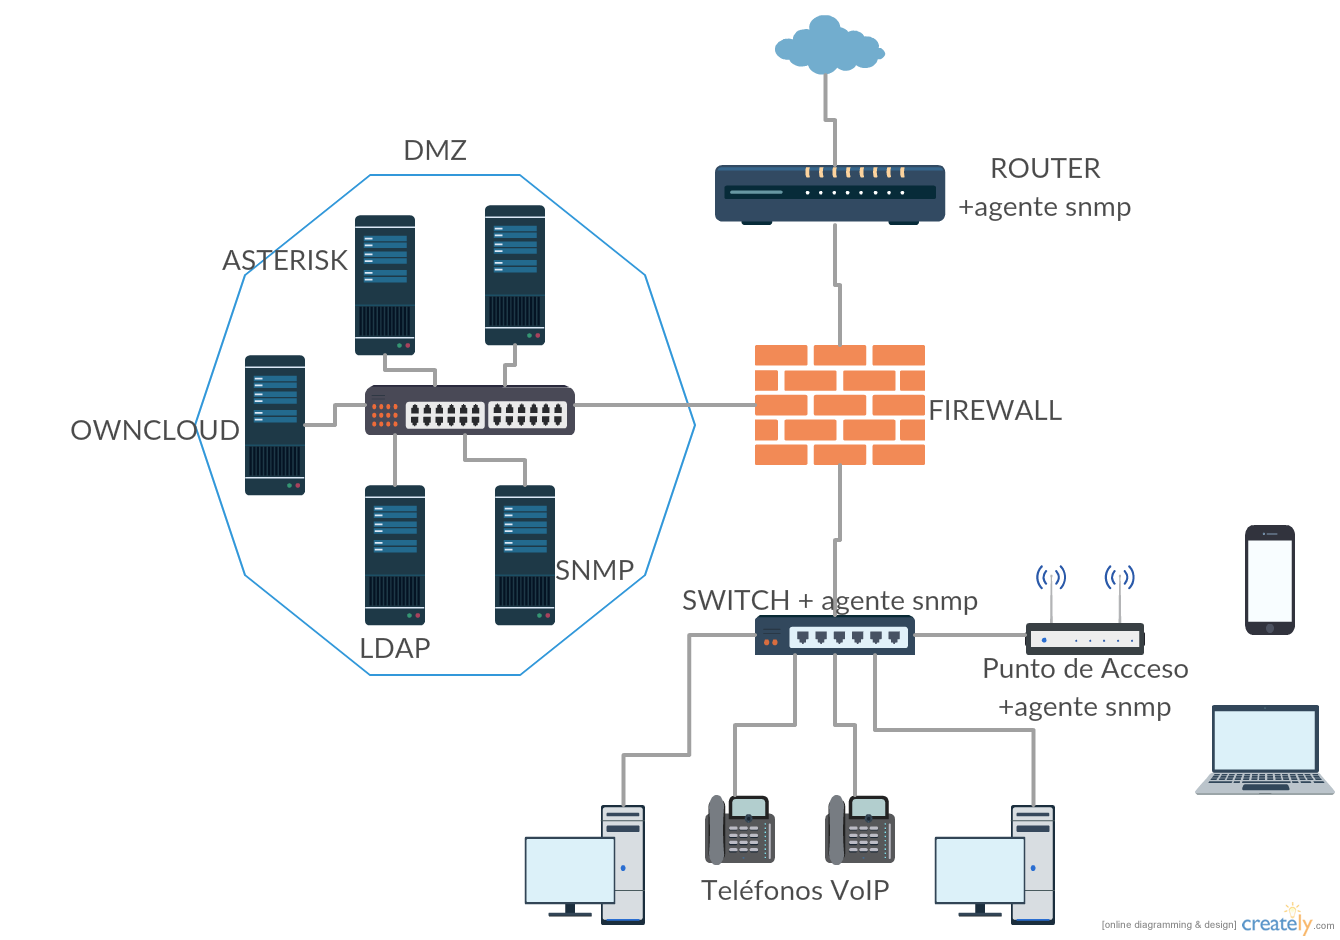
\includegraphics[scale=0.5]{images/topoideal.png}
	\caption{Topología ideal}
	\label{fig:topoideal}
\end{figure}

\subsection{Dispositivos disponibles}

Tenemos para las pruebas y el desarrollo de la práctica, las siguientes herramientas hardware:

\begin{itemize}

	\item Un \textbf{switch} con VLAN y 5 puertos.
	\item Un ordenador que actúa de \textbf{enrutador}, con dos puertos ethernet, uno de ellos con configuración VLAN.
	\item Un \textbf{punto de acceso} WiFi para el acceso a la red.
	\item Un \textbf{iPhone} y un \textbf{portátil Mac}, útiles para probar VOIP con wifi.
	\item Dos ordenadores que actúan como \textbf{organizaciones} 31 y 32.
	\item Dos ordenadores más para simular \textbf{clientes} haciendo peticiones.

\end{itemize}




\subsection{Topología desplegada}

En cuanto a la topología física real, disponemos en el laboratorio de 3 torres, 5 puertos del switch CISCO y un punto de acceso wifi configurado para la organización 31. La conexión de una de las torres como router y las otras dos como equipos de cada organización ya se explica en los boletines de prácticas.

A partir de esa configuración básica, configuramos las dos organizaciones de manera casi simétrica: en la \textbf{máquina física} de cada organización se ejecutarán \textbf{todos los servicios}, es decir, del diseño lógico ideal donde cada servicio tiene una máquina física para él solo, ahora todos los servicios conviven en la misma máquina física. Decidimos usar un servidor físico porque la cantidad de servicios proporcionados por la organización no son tan pesados como \textbf{carga de trabajo} conjunta para una única máquina, como lo pueda ser tener \textbf{varios} servidores como \textbf{máquinas virtuales} en la misma torre del laboratorio.

Ahora bien, por el modo en que programamos la instalación de servicios, nos es muy fácil portarlos desde una máquina física a varias, cambiando las configuraciones de la IP de cada máquina.

En la \autoref{fig:topofisica} vemos el diagrama de la topología física, donde tenemos el ordenador que hace de router, los otros dos ordenadores del laboratorio que actuarán de servidores, el punto de acceso donde usamos nuestros móviles y portátiles personales, y la posibilidad de usar otra torre del laboratorio como cliente.


\begin{figure}[h!]
	\caption{Topología física}
	\centering
		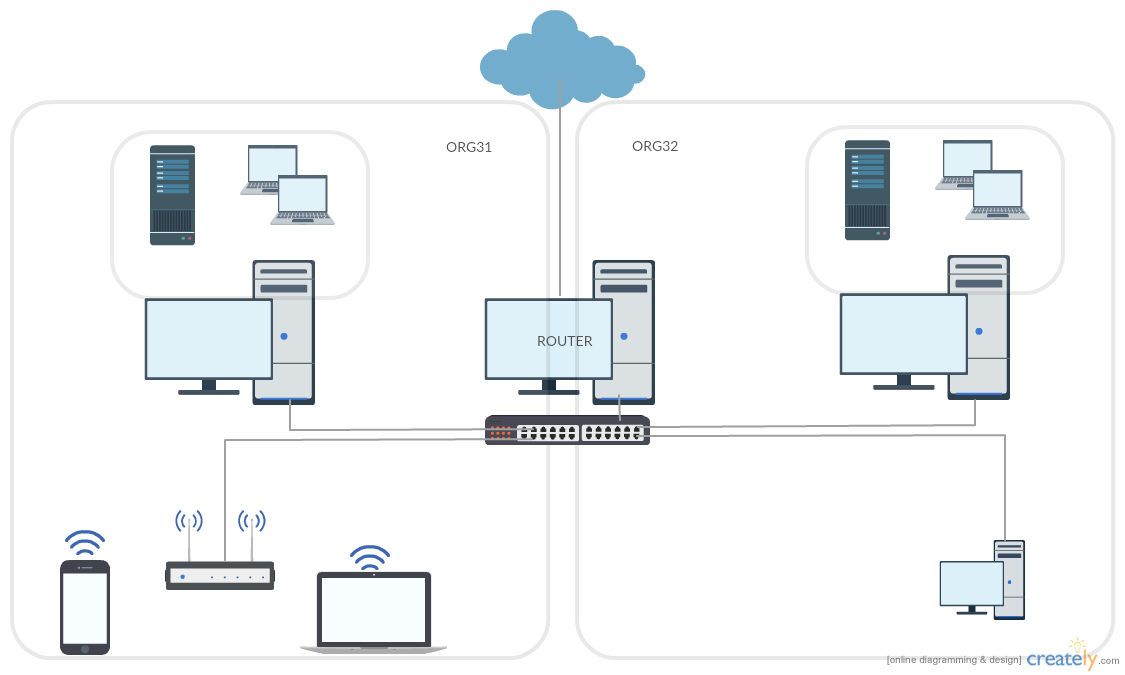
\includegraphics[scale=0.35]{images/TopologiaFisica}
	\label{fig:topofisica}
\end{figure}




\section{Configuración de los dispositivos}

Para la configuración de los dispositivos utilizamos herramientas Makefile, y scripts escritos en bash y python, de manera que desplegar los servicios y la topología en un dispositivo esté automatizado, llegando a tal punto que en la instalación sólo haría falta intervenir para escribir la contraseña de la base de datos de Owncloud y pulsar Intro en alguna instalación. No nos apoyamos en una máquina virtual que vayamos configurando a lo largo de las prácticas llevándola de un lado a otro, y por lo general, usamos máquinas virtuales con una instantánea \textit{limpia}.
\\

Usamos una estructura de directorios basada en el hardware a configurar. Es decir, en el ordenador que hace de enrutador ejecutamos un Makefile que está en el directorio ROUTER; para la máquina servidor de la organización 31, la carpeta SERVER correspondiente; etc.

%TODO: decidir si se pone la estructura, y si se modifica cómo presentarla.
\begin{Verbatim}
ROUTER
	SNMP
	Makefile
	network
	test
ORG1
	FISICA
		Makefile
		network
		test
	SERVER
		SNMP
		VOIP
		Makefile
		network
		test
	CLIENTE1
		SNMP
		VOIP
		Makefile
		network
		test

\end{Verbatim}





\section{Servicios}

\subsection{Enrutamiento}

Del enrutamiento se encarga el PC que hace de router. La configuración física se basa en dos puertos Ethernet y VLAN:

\begin{itemize}
	\item Un puerto se usa para conectarse a la red de la UMu, que da conectividad al exterior.
	\item Otro puerto, conectado al \textit{trunk switch vlan} de la organización 31 y 32.
\end{itemize}

La configuración lógica, es decir, la configuración de los interfaces de red es la siguiente:

\begin{lstlisting}
TODO: Copiar la configuracion de las interfaces.
\end{lstlisting}
\lstinputlisting{../ROUTER/network}
%Explicar fichero

El script instala el soporte de vlan en el ordenador, desactiva el gestor de redes de ubuntu, copia en \textit{/etc/network/interfaces} la configuración de los puertos ethernet: eth0 conexión a la red UMu con DHCP; eth1.31 y eth1.32 las dos VLAN para el segundo puerto ethernet. A continuación, copia en \textit{/etc/hosts} los nombres correspondientes a las IPs de las máquinas de cada organización, para solventar la falta de un servidor DNS que los registre. Hay máquinas de más de cara a posibles expansiones durante el desarrollo de la práctica, ahorrarnos modificar el fichero varias veces. Por último activa el \textit{forwarding} de paquetes y la regla de iptables para actuar como NAT para la subred 192.168.0.0/16, enviando los paquetes por eth0.

En las máquinas servidor basta con modificar el fichero \textit{/etc/network/interfaces} para configurar la IP fija 192.168.3i.100, pues no tenemos servidor DHCP para autoconfiguración.


\subsection{SNMP}

\subsubsection{Agentes}

\subsubsection{Manejador}

\subsection{Voz sobre IP}

En esta sección documentamos las configuraciones que hemos tomado para el servidor de Asterisk.

\subsubsection{Configuración básica}

Para las organizaciones 31 y 32, hacemos 2 cuentas de cliente para ambas organizaciones (311 y 312 para organización 31; 321 y 322 para la organización 32).

\begin{lstlisting}
TODO: Copiar aqui la configuracion relativa a los clientes.
\end{lstlisting}

Para esos clientes también hemos configurado sus extensiones.

\begin{lstlisting}
TODO: Copiar aqui la configuracion relativa a las extensiones.
\end{lstlisting}

\subsubsection{Troncales Asterisk}

Para empezar, hacemos una redirección básica entre los dos servicios Asterisk en las configuraciones de extensión de Asterisk:

\begin{lstlisting}
TODO: Copiar aqui la configuracion relativa a las extensiones entre servicios.
\end{lstlisting}

\subsubsection{Buzón de voz}

\subsection{LDAP}
El servicio LDAP ofrece al resto de servicios un punto en común donde encontrar la información relevante de los usuarios (nombres,
organización a la que pertenecen, permisos de uso y acceso, credenciales, etc).

Como contiene la información crítica de los usuarios que se integran en los servicios, LDAP se despliega en su propia máquina.

Sin embargo, en el despliegue real del laboratorio, LDAP está integrado en el ordenador de la organización 31.

Para las pruebas de laboratorio, la instalación y la configuración la generamos automáticamente (sin necesidad de
interacción del administrador), en python, generando tres clientes de la organización 31.

%TODO: Incluir partes o total del fichero python.
%TODO: Incluir un ldiff y comentarlo.
%TODO: Describir qué es db.tar.gz e initial.tar.gz
%TODO: Justificar que funciona correctamente con ldapsearch.
%TODO: LDAP lo integramos con OwnCloud y lo probamos.

\subsection{OwnCloud}

\section{Políticas de seguridad}
%TODO: Un dibujo del escenario de seguridad

\subsection{Análisis de riesgos}
%TODO: Tabla de reglas de seguridad

\subsection{Configuración de seguridad}
%TODO: Iptables

\subsection{Generación de certificados}
En openssl.cnf no se explica que %yo me entiendo

[ usr_cert ]

crlDistributionPoints = URI:http://server.org31/crl/org31.CRL

\end{document}
